\documentclass[11pt]{article}

% Required Packages
\usepackage{amsmath}
\usepackage{amssymb}
\usepackage{amsthm}
\usepackage{geometry}
\usepackage{mathrsfs}
\usepackage{mathtools}
\usepackage{tikz}
\usepackage[colorlinks=true, linkcolor=blue, linktoc=all]{hyperref}

% Page Geometry
\geometry{letterpaper, margin=1in}

% Theorem Environments
\renewcommand{\qedsymbol}{$\blacksquare$}

% Title Information
\title{\textbf{Rigorous Practice Problem Set: \\ Proofs Involving Real Numbers \& Abstract Modeling}}
\author{Tashfeen Omran}
\date{\today}

\begin{document}

\maketitle

\tableofcontents
\newpage

% ==========================================
\section{Concept Checklist \& Question Mapping}
\label{sec:checklist_start}
% ==========================================
The following checklist details the theoretical concepts, logical structures, and proof techniques extracted from the source material. Every concept is rigorously tested in the accompanying problem set.

\begin{itemize}
    \item \textbf{C1: Algebraic Manipulation \& Direct Proofs (Perfect Squares):} Utilizing the axiom that $x^2 \ge 0$ for all $x \in \mathbb{R}$ to establish bounds. (Problems 1, 2, 3, 4, 5)
    \item \textbf{C2: Proof by Contrapositive:} Transforming ``OR'' disjunctions and strict inequalities into inclusive bounds using De Morgan's Laws. (Problems 6, 7, 8, 9, 10)
    \item \textbf{C3: Absolute Value \& Triangle Inequality:} Employing the ``Adding Zero'' trick and piecewise definitions to bound distances in metric spaces. (Problems 11, 12, 13, 14, 15)
    \item \textbf{C4: Arithmetic-Geometric Mean (AM-GM):} Proving the inequality and establishing the exact conditions for equality. (Problems 16, 17, 18)
    \item \textbf{C5: Cauchy-Schwarz Inequality:} Utilizing the discriminant of a quadratic function to bound inner products in $\mathbb{R}^2$. (Problems 19, 20)
    \item \textbf{C6: Logical Fallacies \& Diagnostic Flaws:} Identifying circular reasoning, invalid sign divisions, and false contrapositives. (Problems 21, 22, 23, 24, 25)
    \item \textbf{C7: Abstract Modeling - Machine Learning (L1 Regularization):} Proving metric properties and parameter space convexity for Lasso regression. (Problems 26, 27)
    \item \textbf{C8: Abstract Modeling - Quantitative Finance (Coherent Risk):} Proving subadditivity and positive homogeneity for $L^2$ risk measures. (Problems 28, 29)
    \item \textbf{C9: Proof by Cases \& Synthesis:} Exhausting real number trichotomy to establish absolute value identities. (Problem 30)
\end{itemize}

\newpage

% ==========================================
\section{Problem Sets}
\label{sec:problems}
% ==========================================

\subsection{Part 1: Algebraic Manipulation and Direct Proofs}
\begin{enumerate}
    \item Prove that for all real numbers $x$ and $y$, $x^2 + y^2 \ge 2xy$.
    \item Prove that for all real numbers $x, y,$ and $z$, $x^2 + y^2 + z^2 \ge xy + yz + zx$.
    \item Prove that for every positive real number $x$, $x + \frac{9}{x} \ge 6$.
    \item Let $x, y \in \mathbb{R}$. Prove that if $x^2 - 6x = y^2 - 6y$ and $x \neq y$, then $x + y = 6$.
    \item Prove that if $r$ is a real number such that $0 < r < 1$, then $\frac{1}{r(1-r)} \ge 4$.
\end{enumerate}

\subsection{Part 2: Proof by Contrapositive}
\begin{enumerate}
    \setcounter{enumi}{5}
    \item Prove that if $x \in \mathbb{R}$ and $x^2 - 7x + 12 < 0$, then $x > 0$.
    \item Let $a$ and $b$ be integers. Prove that if $5a + 7b \ge 35$, then $a \ge 3$ or $b \ge 3$.
    \item Let $x \in \mathbb{R}$. Prove that if $x^4 + 1 \le x^7 + x^3$, then $x > 0$.
    \item Prove that for any real number $x$, if $x^3 < 0$, then $x < 0$.
    \item Prove that if $x, y \in \mathbb{R}$ and $x + y > 100$, then $x > 50$ or $y > 50$.
\end{enumerate}

\subsection{Part 3: Absolute Values and Triangle Inequality}
\begin{enumerate}
    \setcounter{enumi}{10}
    \item Prove for every three real numbers $x, y,$ and $z$ that $|x - y| \le |x - z| + |z - y|$.
    \item Prove the Reverse Triangle Inequality: For all $x, y \in \mathbb{R}$, $|x| - |y| \le |x - y|$.
    \item Extend the previous result to prove that for all $x, y \in \mathbb{R}$, $||x| - |y|| \le |x - y|$.
    \item Prove that for all $x, y, z \in \mathbb{R}$, $|x + y + z| \le |x| + |y| + |z|$.
    \item Prove that if $x, y, c \in \mathbb{R}$ and $|x - y| < c$, then $|x| < |y| + c$.
\end{enumerate}

\subsection{Part 4: Means (AM-GM) and Cauchy-Schwarz}
\begin{enumerate}
    \setcounter{enumi}{15}
    \item Prove that for any positive real numbers $a$ and $b$, $\sqrt{ab} \le \frac{a+b}{2}$.
    \item Prove that for any positive real numbers $x$ and $y$, $(x+y)\left(\frac{1}{x} + \frac{1}{y}\right) \ge 4$.
    \item Prove that for any positive real numbers $a, b,$ and $c$, $(a+b)(b+c)(c+a) \ge 8abc$.
    \item Consider the function $f(t) = (at - x)^2 + (bt - y)^2$. By analyzing the discriminant of this quadratic in $t$, prove the Cauchy-Schwarz Inequality in $\mathbb{R}^2$: $(ax + by)^2 \le (a^2 + b^2)(x^2 + y^2)$.
    \item Use the Cauchy-Schwarz Inequality to prove that for any $x, y \in \mathbb{R}$, $x + 2y \le \sqrt{5(x^2 + y^2)}$.
\end{enumerate}

\subsection{Part 5: Advanced Diagnostic Testing (Find the Flaw)}
\textit{For each of the following, identify the logical or mathematical flaw, explain why it is invalid, and provide the correct logical step or state if the original premise is false.}
\begin{enumerate}
    \setcounter{enumi}{20}
    \item \textbf{Flawed Proof A:} ``Prove that if $x^2 > y^2$, then $x > y$. \textit{Proof:} Take the square root of both sides to get $\sqrt{x^2} > \sqrt{y^2}$. Since the square root cancels the square, $x > y$.''
    \item \textbf{Flawed Proof B:} ``Prove for $x > 0$ that $x + \frac{1}{x} \ge 2$. \textit{Proof:} $x + \frac{1}{x} \ge 2 \implies x^2 + 1 \ge 2x \implies x^2 - 2x + 1 \ge 0 \implies (x-1)^2 \ge 0$. Since squares are non-negative, the statement is true.''
    \item \textbf{Flawed Proof C:} ``Prove $|x - y| \le |x| - |y|$. \textit{Proof:} By the Triangle Inequality, $|a + b| \le |a| + |b|$. Let $a = x$ and $b = -y$. Then $|x + (-y)| \le |x| + |-y|$. Since $|-y| = -|y|$, we get $|x - y| \le |x| - |y|$.''
    \item \textbf{Flawed Proof D:} ``Prove if $ab = 0$, then $a = 0$ and $b = 0$. \textit{Proof:} If $a = 0$, then $0 \cdot b = 0$, which is true. If $b = 0$, then $a \cdot 0 = 0$, which is true. Thus $a = 0$ and $b = 0$.''
    \item \textbf{Flawed Proof E:} ``Prove if $x < 0$, then $x^3 < 0$. \textit{Proof:} We use the contrapositive: 'If $x > 0$, then $x^3 > 0$'. Assume $x > 0$. Multiplying by $x^2$ (which is positive) gives $x^3 > 0$. Thus the original statement is true.''
\end{enumerate}

\subsection{Part 6: Abstract Real-World Modeling \& Synthesis}
\begin{enumerate}
    \setcounter{enumi}{25}
    \item \textbf{Machine Learning (L1 Regularization):} Let $w = (w_1, w_2)$ and $v = (v_1, v_2)$ be weight vectors in $\mathbb{R}^2$. Define the L1 norm as $\|w\|_1 = |w_1| + |w_2|$. Prove that the L1 norm satisfies the Triangle Inequality: $\|w + v\|_1 \le \|w\|_1 + \|v\|_1$.
    \item \textbf{Machine Learning (Convexity):} A parameter space $S$ is convex if for any $u, v \in S$ and any $t \in [0, 1]$, the vector $tu + (1-t)v \in S$. Prove that the L1 penalty space $S = \{w \in \mathbb{R}^2 : \|w\|_1 \le 1\}$ is convex.
    \item \textbf{Quant Finance (Positive Homogeneity):} Let $X$ be a random variable representing portfolio returns. Define the $L^2$ risk measure as $\rho(X) = \sqrt{\mathbb{E}[X^2]}$. Prove that for any constant $c > 0$, $\rho(cX) = c\rho(X)$.
    \item \textbf{Quant Finance (Subadditivity):} Assume the expectation operator is linear ($\mathbb{E}[X+Y] = \mathbb{E}[X] + \mathbb{E}[Y]$) and satisfies the stochastic Cauchy-Schwarz inequality $\mathbb{E}[XY] \le \sqrt{\mathbb{E}[X^2]\mathbb{E}[Y^2]}$. Prove that the risk measure $\rho(X) = \sqrt{\mathbb{E}[X^2]}$ is subadditive: $\rho(X + Y) \le \rho(X) + \rho(Y)$.
    \item \textbf{Synthesis (Proof by Cases):} Prove that for any real numbers $x$ and $y$, the maximum of the two numbers can be expressed algebraically as $\max(x, y) = \frac{x + y + |x - y|}{2}$.
\end{enumerate}

\newpage

% ==========================================
\section{Detailed Solutions}
\label{sec:solutions}
% ==========================================

\begin{proof}[Solution to Problem 1]
    \textbf{Method: Direct Proof.} \\
    Assume $x, y \in \mathbb{R}$. By the positivity axioms of real numbers, the square of any real number is non-negative. Consider the real number $(x - y)$. We have:
    \[ (x - y)^2 \ge 0 \]
    Expanding the binomial yields:
    \[ x^2 - 2xy + y^2 \ge 0 \]
    Adding $2xy$ to both sides gives:
    \[ x^2 + y^2 \ge 2xy \]
    This completes the proof.
\end{proof}

\begin{proof}[Solution to Problem 2]
    \textbf{Method: Direct Proof.} \\
    Assume $x, y, z \in \mathbb{R}$. We know that the sum of squares is non-negative. Therefore:
    \[ (x - y)^2 + (y - z)^2 + (z - x)^2 \ge 0 \]
    Expanding each binomial yields:
    \[ (x^2 - 2xy + y^2) + (y^2 - 2yz + z^2) + (z^2 - 2zx + x^2) \ge 0 \]
    Combining like terms:
    \[ 2x^2 + 2y^2 + 2z^2 - 2xy - 2yz - 2zx \ge 0 \]
    Adding the cross terms to the right side:
    \[ 2x^2 + 2y^2 + 2z^2 \ge 2xy + 2yz + 2zx \]
    Dividing the entire inequality by 2 (which preserves the inequality sign since $2 > 0$) yields:
    \[ x^2 + y^2 + z^2 \ge xy + yz + zx \]
    This completes the proof.
\end{proof}

\begin{proof}[Solution to Problem 3]
    \textbf{Method: Direct Proof.} \\
    Assume $x \in \mathbb{R}$ and $x > 0$. Consider the real number $(x - 3)$. Its square is non-negative:
    \[ (x - 3)^2 \ge 0 \]
    Expanding the square yields:
    \[ x^2 - 6x + 9 \ge 0 \]
    Adding $6x$ to both sides gives:
    \[ x^2 + 9 \ge 6x \]
    Since we are given $x > 0$, we can divide both sides by $x$ without changing the direction of the inequality:
    \[ \frac{x^2 + 9}{x} \ge \frac{6x}{x} \]
    Simplifying the fractions yields:
    \[ x + \frac{9}{x} \ge 6 \]
    This completes the proof.
\end{proof}

\begin{proof}[Solution to Problem 4]
    \textbf{Method: Direct Proof.} \\
    Assume $x, y \in \mathbb{R}$ such that $x^2 - 6x = y^2 - 6y$ and $x \neq y$. We rearrange the equation to group quadratic and linear terms:
    \[ x^2 - y^2 - 6x + 6y = 0 \]
    Factoring the difference of squares and factoring out $-6$ from the linear terms:
    \[ (x - y)(x + y) - 6(x - y) = 0 \]
    Factoring out the common binomial $(x - y)$:
    \[ (x - y)(x + y - 6) = 0 \]
    By the Zero Product Property, either $x - y = 0$ or $x + y - 6 = 0$. Since we are given $x \neq y$, it follows that $x - y \neq 0$. Therefore, the second factor must be zero:
    \[ x + y - 6 = 0 \implies x + y = 6 \]
    This completes the proof.
\end{proof}

\begin{proof}[Solution to Problem 5]
    \textbf{Method: Direct Proof (via algebraic equivalence).} \\
    Assume $r \in \mathbb{R}$ and $0 < r < 1$. This implies $r > 0$ and $1 - r > 0$, so their product $r(1 - r) > 0$. We start with a known axiomatic truth. Since $2r - 1 \in \mathbb{R}$, its square is non-negative:
    \[ (2r - 1)^2 \ge 0 \]
    Expanding the square:
    \[ 4r^2 - 4r + 1 \ge 0 \]
    Rearranging terms:
    \[ 1 \ge 4r - 4r^2 \]
    Factoring out $4r$ on the right side:
    \[ 1 \ge 4r(1 - r) \]
    Since $r(1 - r) > 0$, we can divide both sides by $r(1 - r)$ without flipping the inequality:
    \[ \frac{1}{r(1 - r)} \ge 4 \]
    This completes the proof.
\end{proof}

\begin{proof}[Solution to Problem 6]
    \textbf{Method: Proof by Contrapositive.} \\
    The statement is $P \implies Q$. We will prove $\sim Q \implies \sim P$. The contrapositive is: ``If $x \le 0$, then $x^2 - 7x + 12 \ge 0$.'' \\
    Assume $x \le 0$. Since $x \le 0$, multiplying by $-7$ (a negative number) flips the inequality, yielding $-7x \ge 0$. Furthermore, the square of any real number is non-negative, so $x^2 \ge 0$. \\
    Adding these non-negative terms together with 12 gives:
    \[ x^2 - 7x + 12 \ge 0 + 0 + 12 = 12 \]
    Since $12 \ge 0$, by transitivity, $x^2 - 7x + 12 \ge 0$. This proves the contrapositive, establishing the original statement.
\end{proof}

\begin{proof}[Solution to Problem 7]
    \textbf{Method: Proof by Contrapositive.} \\
    The conclusion is a disjunction ($a \ge 3 \lor b \ge 3$). By De Morgan's Laws, the negation is $(a < 3 \land b < 3)$. Since $a$ and $b$ are integers, $a < 3 \implies a \le 2$ and $b < 3 \implies b \le 2$. \\
    The contrapositive statement is: ``If $a \le 2$ and $b \le 2$, then $5a + 7b < 35$.'' \\
    Assume $a \le 2$ and $b \le 2$. Multiplying by positive constants:
    \[ 5a \le 10 \quad \text{and} \quad 7b \le 14 \]
    Adding these inequalities yields:
    \[ 5a + 7b \le 10 + 14 = 24 \]
    Since $24 < 35$, it follows that $5a + 7b < 35$. The contrapositive is true, so the original statement is true.
\end{proof}

\begin{proof}[Solution to Problem 8]
    \textbf{Method: Proof by Contrapositive.} \\
    The contrapositive is: ``If $x \le 0$, then $x^4 + 1 > x^7 + x^3$.'' \\
    Assume $x \le 0$. Any odd power of a non-positive number is non-positive, so $x^7 \le 0$ and $x^3 \le 0$. Adding these gives:
    \[ x^7 + x^3 \le 0 \]
    Any even power of a real number is non-negative, so $x^4 \ge 0$. Adding 1 gives:
    \[ x^4 + 1 \ge 1 > 0 \]
    By transitivity, since $x^4 + 1 > 0$ and $0 \ge x^7 + x^3$, we conclude:
    \[ x^4 + 1 > x^7 + x^3 \]
    This proves the contrapositive.
\end{proof}

\begin{proof}[Solution to Problem 9]
    \textbf{Method: Proof by Contrapositive.} \\
    The contrapositive is: ``If $x \ge 0$, then $x^3 \ge 0$.'' \\
    Assume $x \ge 0$. We proceed by cases. \\
    \textit{Case 1:} $x = 0$. Then $x^3 = 0^3 = 0$. Thus $x^3 \ge 0$ holds. \\
    \textit{Case 2:} $x > 0$. The product of positive numbers is positive. Since $x > 0$, $x \cdot x \cdot x = x^3 > 0$. Thus $x^3 \ge 0$ holds. \\
    In all cases, the contrapositive is true, which implies the original statement is true.
\end{proof}

\begin{proof}[Solution to Problem 10]
    \textbf{Method: Proof by Contrapositive.} \\
    The conclusion is $x > 50 \lor y > 50$. By De Morgan's Laws, the negation is $x \le 50 \land y \le 50$. \\
    The contrapositive is: ``If $x \le 50$ and $y \le 50$, then $x + y \le 100$.'' \\
    Assume $x \le 50$ and $y \le 50$. Adding these two inequalities yields:
    \[ x + y \le 50 + 50 = 100 \]
    This exactly matches the negated premise. The contrapositive is proven.
\end{proof}

\begin{proof}[Solution to Problem 11]
    \textbf{Method: Direct Proof (Adding Zero).} \\
    Assume $x, y, z \in \mathbb{R}$. We wish to bound $|x - y|$. We introduce $z$ by adding and subtracting it inside the absolute value:
    \[ |x - y| = |x - z + z - y| \]
    Let $a = x - z$ and $b = z - y$. By the standard Triangle Inequality ($|a + b| \le |a| + |b|$), we have:
    \[ |(x - z) + (z - y)| \le |x - z| + |z - y| \]
    Therefore, $|x - y| \le |x - z| + |z - y|$.
\end{proof}

\begin{proof}[Solution to Problem 12]
    \textbf{Method: Direct Proof (Triangle Inequality).} \\
    Assume $x, y \in \mathbb{R}$. We can express $x$ as $(x - y) + y$. Taking the absolute value:
    \[ |x| = |(x - y) + y| \]
    Applying the Triangle Inequality where $a = x - y$ and $b = y$:
    \[ |x| \le |x - y| + |y| \]
    Subtracting $|y|$ from both sides yields:
    \[ |x| - |y| \le |x - y| \]
    This completes the proof.
\end{proof}

\begin{proof}[Solution to Problem 13]
    \textbf{Method: Direct Proof (Symmetry).} \\
    Assume $x, y \in \mathbb{R}$. From Problem 12, we established:
    \[ |x| - |y| \le |x - y| \quad \text{(Equation 1)} \]
    By swapping the roles of $x$ and $y$, we also have:
    \[ |y| - |x| \le |y - x| \]
    Since $|y - x| = |-(x - y)| = |x - y|$, this becomes:
    \[ -(|x| - |y|) \le |x - y| \quad \text{(Equation 2)} \]
    Recall the property of absolute values: $|A| \le B \iff -B \le A \le B$. Equations 1 and 2 state exactly that $-|x - y| \le |x| - |y| \le |x - y|$. Therefore:
    \[ ||x| - |y|| \le |x - y| \]
\end{proof}

\begin{proof}[Solution to Problem 14]
    \textbf{Method: Direct Proof (Iterated Triangle Inequality).} \\
    Assume $x, y, z \in \mathbb{R}$. Group the terms as $(x + y)$ and $z$. Applying the Triangle Inequality:
    \[ |(x + y) + z| \le |x + y| + |z| \]
    Now apply the Triangle Inequality again to $|x + y|$:
    \[ |x + y| \le |x| + |y| \]
    Substituting this bound into the first inequality yields:
    \[ |x + y + z| \le |x| + |y| + |z| \]
\end{proof}

\begin{proof}[Solution to Problem 15]
    \textbf{Method: Direct Proof.} \\
    Assume $x, y, c \in \mathbb{R}$ and $|x - y| < c$. By the Triangle Inequality (as shown in Problem 12), we know:
    \[ |x| - |y| \le |x - y| \]
    Since we are given $|x - y| < c$, we can use transitivity:
    \[ |x| - |y| < c \]
    Adding $|y|$ to both sides yields:
    \[ |x| < |y| + c \]
    This completes the proof.
\end{proof}

\begin{proof}[Solution to Problem 16]
    \textbf{Method: Direct Proof.} \\
    Assume $a, b > 0$. Consider the real numbers $\sqrt{a}$ and $\sqrt{b}$. The square of their difference is non-negative:
    \[ (\sqrt{a} - \sqrt{b})^2 \ge 0 \]
    Expanding the square:
    \[ a - 2\sqrt{ab} + b \ge 0 \]
    Adding $2\sqrt{ab}$ to both sides:
    \[ a + b \ge 2\sqrt{ab} \]
    Dividing by 2 yields the AM-GM inequality:
    \[ \frac{a + b}{2} \ge \sqrt{ab} \]
\end{proof}

\begin{proof}[Solution to Problem 17]
    \textbf{Method: Direct Proof.} \\
    Assume $x, y > 0$. Expand the product:
    \[ (x + y)\left(\frac{1}{x} + \frac{1}{y}\right) = 1 + \frac{x}{y} + \frac{y}{x} + 1 = 2 + \frac{x}{y} + \frac{y}{x} \]
    We must show that $\frac{x}{y} + \frac{y}{x} \ge 2$. Since $x, y > 0$, $\frac{x}{y}$ and $\frac{y}{x}$ are positive. Applying the AM-GM inequality (Problem 16) to $a = \frac{x}{y}$ and $b = \frac{y}{x}$:
    \[ \frac{x}{y} + \frac{y}{x} \ge 2\sqrt{\left(\frac{x}{y}\right)\left(\frac{y}{x}\right)} = 2\sqrt{1} = 2 \]
    Substituting this back into our expanded equation:
    \[ 2 + \left(\frac{x}{y} + \frac{y}{x}\right) \ge 2 + 2 = 4 \]
    This completes the proof.
\end{proof}

\begin{proof}[Solution to Problem 18]
    \textbf{Method: Direct Proof (Multiple AM-GM Applications).} \\
    Assume $a, b, c > 0$. By the AM-GM inequality, we can establish three separate bounds:
    \[ a + b \ge 2\sqrt{ab} \]
    \[ b + c \ge 2\sqrt{bc} \]
    \[ c + a \ge 2\sqrt{ca} \]
    Since $a, b, c > 0$, all terms on both sides of these inequalities are strictly positive. We can multiply these three inequalities together without changing the inequality direction:
    \[ (a + b)(b + c)(c + a) \ge (2\sqrt{ab})(2\sqrt{bc})(2\sqrt{ca}) \]
    Simplifying the right side:
    \[ 8\sqrt{a^2 b^2 c^2} = 8abc \]
    Thus, $(a + b)(b + c)(c + a) \ge 8abc$.
\end{proof}

\begin{proof}[Solution to Problem 19]
    \textbf{Method: Direct Proof (Discriminant Analysis).} \\
    Assume $a, b, x, y \in \mathbb{R}$. Define $f(t) = (at - x)^2 + (bt - y)^2$ for $t \in \mathbb{R}$. Since $f(t)$ is a sum of squares, $f(t) \ge 0$ for all $t$. Expanding $f(t)$:
    \[ f(t) = a^2 t^2 - 2axt + x^2 + b^2 t^2 - 2byt + y^2 \]
    Grouping by powers of $t$:
    \[ f(t) = (a^2 + b^2)t^2 - 2(ax + by)t + (x^2 + y^2) \]
    This is a quadratic in $t$ of the form $At^2 + Bt + C \ge 0$, where $A = a^2 + b^2$, $B = -2(ax + by)$, and $C = x^2 + y^2$. For a quadratic to be non-negative for all real $t$, it cannot have two distinct real roots. Thus, its discriminant $\Delta = B^2 - 4AC$ must be less than or equal to zero:
    \[ (-2(ax + by))^2 - 4(a^2 + b^2)(x^2 + y^2) \le 0 \]
    \[ 4(ax + by)^2 - 4(a^2 + b^2)(x^2 + y^2) \le 0 \]
    Dividing by 4 and rearranging yields the Cauchy-Schwarz Inequality:
    \[ (ax + by)^2 \le (a^2 + b^2)(x^2 + y^2) \]
\end{proof}

\begin{proof}[Solution to Problem 20]
    \textbf{Method: Direct Proof (Cauchy-Schwarz Application).} \\
    Assume $x, y \in \mathbb{R}$. We apply the Cauchy-Schwarz Inequality $(ax + by)^2 \le (a^2 + b^2)(x^2 + y^2)$ by setting $a = 1$ and $b = 2$:
    \[ (1 \cdot x + 2 \cdot y)^2 \le (1^2 + 2^2)(x^2 + y^2) \]
    \[ (x + 2y)^2 \le 5(x^2 + y^2) \]
    Taking the square root of both sides. Since $\sqrt{u^2} = |u|$ and $|u| \ge u$ for all real $u$:
    \[ x + 2y \le |x + 2y| \le \sqrt{5(x^2 + y^2)} \]
    This completes the proof.
\end{proof}

\begin{proof}[Solution to Problem 21]
    \textbf{Flaw Identification \& Correction.} \\
    \textbf{The Flaw:} The assertion that $\sqrt{x^2} = x$ is false for negative numbers. The correct identity is $\sqrt{x^2} = |x|$. \\
    \textbf{Why it's an error:} If $x = -3$ and $y = 2$, then $(-3)^2 > 2^2$ ($9 > 4$), but $-3$ is not greater than $2$. \\
    \textbf{Correction:} The original statement is false. The corrected theorem should state: ``If $x^2 > y^2$, then $|x| > |y|$.''
\end{proof}

\begin{proof}[Solution to Problem 22]
    \textbf{Flaw Identification \& Correction.} \\
    \textbf{The Flaw:} Circular reasoning (Assuming the Consequent). The proof starts with the target inequality and works backward to a known truth. \\
    \textbf{Why it's an error:} Logical implications do not automatically reverse. $P \implies Q$ being true does not mean $Q \implies P$ is true. \\
    \textbf{Correction:} The proof must be written in reverse. Start with the known truth: ``Since $x \in \mathbb{R}$, $(x - 1)^2 \ge 0$. Expanding gives $x^2 - 2x + 1 \ge 0 \implies x^2 + 1 \ge 2x$. Since $x > 0$, divide by $x$ to get $x + \frac{1}{x} \ge 2$.''
\end{proof}

\begin{proof}[Solution to Problem 23]
    \textbf{Flaw Identification \& Correction.} \\
    \textbf{The Flaw:} The algebraic substitution $|-y| = -|y|$ is mathematically false. \\
    \textbf{Why it's an error:} Absolute value is strictly non-negative. $|-y| = |y|$. For example, if $y = 5$, $|-5| = 5$, but $-|5| = -5$. \\
    \textbf{Correction:} The correct application of the Triangle Inequality yields $|x - y| \le |x| + |y|$. The original statement $|x - y| \le |x| - |y|$ is false (e.g., $x=0, y=1 \implies 1 \le -1$, which is false).
\end{proof}

\begin{proof}[Solution to Problem 24]
    \textbf{Flaw Identification \& Correction.} \\
    \textbf{The Flaw:} The proof confuses the logical ``OR'' with ``AND'', and attempts to prove an implication by assuming the conclusion. \\
    \textbf{Why it's an error:} The Zero Product Property states $ab = 0 \implies a = 0 \lor b = 0$. The statement ``$a = 0 \land b = 0$'' is false (e.g., $a=5, b=0$ gives $ab=0$). \\
    \textbf{Correction:} The original statement is false. The correct theorem is $ab = 0 \implies a = 0 \lor b = 0$.
\end{proof}

\begin{proof}[Solution to Problem 25]
    \textbf{Flaw Identification \& Correction.} \\
    \textbf{The Flaw:} The contrapositive was formed incorrectly. \\
    \textbf{Why it's an error:} The negation of $x < 0$ is $x \ge 0$, not $x > 0$. \\
    \textbf{Correction:} The correct contrapositive is: ``If $x \ge 0$, then $x^3 \ge 0$.'' The proof should proceed: Assume $x \ge 0$. If $x = 0$, $x^3 = 0 \ge 0$. If $x > 0$, $x^3 > 0 \ge 0$. Thus $x^3 \ge 0$.
\end{proof}

\begin{proof}[Solution to Problem 26]
    \textbf{Method: Direct Proof (Triangle Inequality in $\mathbb{R}^2$).} \\
    Assume $w = (w_1, w_2)$ and $v = (v_1, v_2)$. We evaluate $\|w + v\|_1$:
    \[ \|w + v\|_1 = |w_1 + v_1| + |w_2 + v_2| \]
    By the standard Triangle Inequality for real numbers, $|w_1 + v_1| \le |w_1| + |v_1|$ and $|w_2 + v_2| \le |w_2| + |v_2|$. Substituting these bounds:
    \[ \|w + v\|_1 \le (|w_1| + |v_1|) + (|w_2| + |v_2|) \]
    Rearranging the terms:
    \[ \|w + v\|_1 \le (|w_1| + |w_2|) + (|v_1| + |v_2|) = \|w\|_1 + \|v\|_1 \]
    This completes the proof.
\end{proof}

\begin{proof}[Solution to Problem 27]
    \textbf{Method: Direct Proof (Convexity Definition).} \\
    Assume $u, v \in S$, which means $\|u\|_1 \le 1$ and $\|v\|_1 \le 1$. Let $t \in [0, 1]$. We must show that $\|tu + (1-t)v\|_1 \le 1$. \\
    By the Triangle Inequality established in Problem 26:
    \[ \|tu + (1-t)v\|_1 \le \|tu\|_1 + \|(1-t)v\|_1 \]
    By the properties of absolute values, scalars can be factored out: $\|tu\|_1 = |t|\|u\|_1$. Since $t \in [0, 1]$, $t \ge 0$ and $(1-t) \ge 0$, so $|t| = t$ and $|1-t| = 1-t$.
    \[ \|tu + (1-t)v\|_1 \le t\|u\|_1 + (1-t)\|v\|_1 \]
    Since $\|u\|_1 \le 1$ and $\|v\|_1 \le 1$:
    \[ t\|u\|_1 + (1-t)\|v\|_1 \le t(1) + (1-t)(1) = t + 1 - t = 1 \]
    Thus, $tu + (1-t)v \in S$. The set is convex.
    
    \begin{center}
    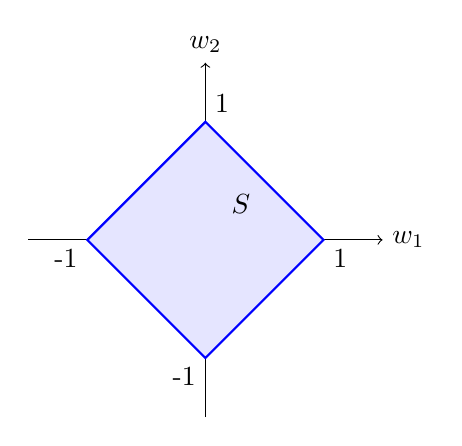
\begin{tikzpicture}[scale=1.5]
        % Draw axes
        \draw[->] (-1.5,0) -- (1.5,0) node[right] {$w_1$};
        \draw[->] (0,-1.5) -- (0,1.5) node[above] {$w_2$};
        % Draw L1 ball
        \draw[thick, blue, fill=blue!10] (1,0) -- (0,1) -- (-1,0) -- (0,-1) -- cycle;
        % Labels
        \node[below right] at (1,0) {1};
        \node[above right] at (0,1) {1};
        \node[below left] at (-1,0) {-1};
        \node[below left] at (0,-1) {-1};
        \node at (0.3, 0.3) {$S$};
    \end{tikzpicture}
    \end{center}
\end{proof}

\begin{proof}[Solution to Problem 28]
    \textbf{Method: Direct Proof.} \\
    Assume $c > 0$. We evaluate $\rho(cX)$:
    \[ \rho(cX) = \sqrt{\mathbb{E}[(cX)^2]} = \sqrt{\mathbb{E}[c^2 X^2]} \]
    By the linearity of expectation, constants can be factored out:
    \[ \sqrt{c^2 \mathbb{E}[X^2]} = \sqrt{c^2} \sqrt{\mathbb{E}[X^2]} \]
    Since $\sqrt{c^2} = |c|$ and $c > 0$, $|c| = c$. Therefore:
    \[ c\sqrt{\mathbb{E}[X^2]} = c\rho(X) \]
    This completes the proof.
\end{proof}

\begin{proof}[Solution to Problem 29]
    \textbf{Method: Direct Proof (Minkowski's Inequality for $p=2$).} \\
    We wish to prove $\rho(X + Y) \le \rho(X) + \rho(Y)$. Since both sides are non-negative, this is equivalent to proving their squares maintain the inequality:
    \[ \rho(X + Y)^2 \le (\rho(X) + \rho(Y))^2 \]
    Expanding the left side using linearity of expectation:
    \[ \rho(X + Y)^2 = \mathbb{E}[(X + Y)^2] = \mathbb{E}[X^2 + 2XY + Y^2] = \mathbb{E}[X^2] + 2\mathbb{E}[XY] + \mathbb{E}[Y^2] \]
    By the given stochastic Cauchy-Schwarz inequality, $\mathbb{E}[XY] \le \sqrt{\mathbb{E}[X^2]}\sqrt{\mathbb{E}[Y^2]} = \rho(X)\rho(Y)$. Substituting this bound:
    \[ \mathbb{E}[X^2] + 2\mathbb{E}[XY] + \mathbb{E}[Y^2] \le \rho(X)^2 + 2\rho(X)\rho(Y) + \rho(Y)^2 \]
    The right side factors into a perfect square:
    \[ \rho(X + Y)^2 \le (\rho(X) + \rho(Y))^2 \]
    Taking the square root of both sides yields $\rho(X + Y) \le \rho(X) + \rho(Y)$.
\end{proof}

\begin{proof}[Solution to Problem 30]
    \textbf{Method: Proof by Cases.} \\
    Assume $x, y \in \mathbb{R}$. By the trichotomy property, either $x \ge y$ or $x < y$. \\
    \textit{Case 1:} Assume $x \ge y$. Then $\max(x, y) = x$. Furthermore, $x - y \ge 0$, so $|x - y| = x - y$. Substituting this into the formula:
    \[ \frac{x + y + |x - y|}{2} = \frac{x + y + (x - y)}{2} = \frac{2x}{2} = x \]
    Thus, the formula holds for Case 1. \\
    \textit{Case 2:} Assume $x < y$. Then $\max(x, y) = y$. Furthermore, $x - y < 0$, so $|x - y| = -(x - y) = y - x$. Substituting this into the formula:
    \[ \frac{x + y + |x - y|}{2} = \frac{x + y + (y - x)}{2} = \frac{2y}{2} = y \]
    Thus, the formula holds for Case 2. \\
    Since the formula holds in all possible cases, $\max(x, y) = \frac{x + y + |x - y|}{2}$ for all $x, y \in \mathbb{R}$.
\end{proof}

\newpage

% ==========================================
\section{Concept Checklist \& Question Mapping (Repeated)}
\label{sec:checklist_end}
% ==========================================
\begin{itemize}
    \item \textbf{C1: Algebraic Manipulation \& Direct Proofs (Perfect Squares):} Utilizing the axiom that $x^2 \ge 0$ for all $x \in \mathbb{R}$ to establish bounds. (Problems 1, 2, 3, 4, 5)
    \item \textbf{C2: Proof by Contrapositive:} Transforming ``OR'' disjunctions and strict inequalities into inclusive bounds using De Morgan's Laws. (Problems 6, 7, 8, 9, 10)
    \item \textbf{C3: Absolute Value \& Triangle Inequality:} Employing the ``Adding Zero'' trick and piecewise definitions to bound distances in metric spaces. (Problems 11, 12, 13, 14, 15)
    \item \textbf{C4: Arithmetic-Geometric Mean (AM-GM):} Proving the inequality and establishing the exact conditions for equality. (Problems 16, 17, 18)
    \item \textbf{C5: Cauchy-Schwarz Inequality:} Utilizing the discriminant of a quadratic function to bound inner products in $\mathbb{R}^2$. (Problems 19, 20)
    \item \textbf{C6: Logical Fallacies \& Diagnostic Flaws:} Identifying circular reasoning, invalid sign divisions, and false contrapositives. (Problems 21, 22, 23, 24, 25)
    \item \textbf{C7: Abstract Modeling - Machine Learning (L1 Regularization):} Proving metric properties and parameter space convexity for Lasso regression. (Problems 26, 27)
    \item \textbf{C8: Abstract Modeling - Quantitative Finance (Coherent Risk):} Proving subadditivity and positive homogeneity for $L^2$ risk measures. (Problems 28, 29)
    \item \textbf{C9: Proof by Cases \& Synthesis:} Exhausting real number trichotomy to establish absolute value identities. (Problem 30)
\end{itemize}

\end{document}